\documentclass[tikz]{standalone}
\begin{document}
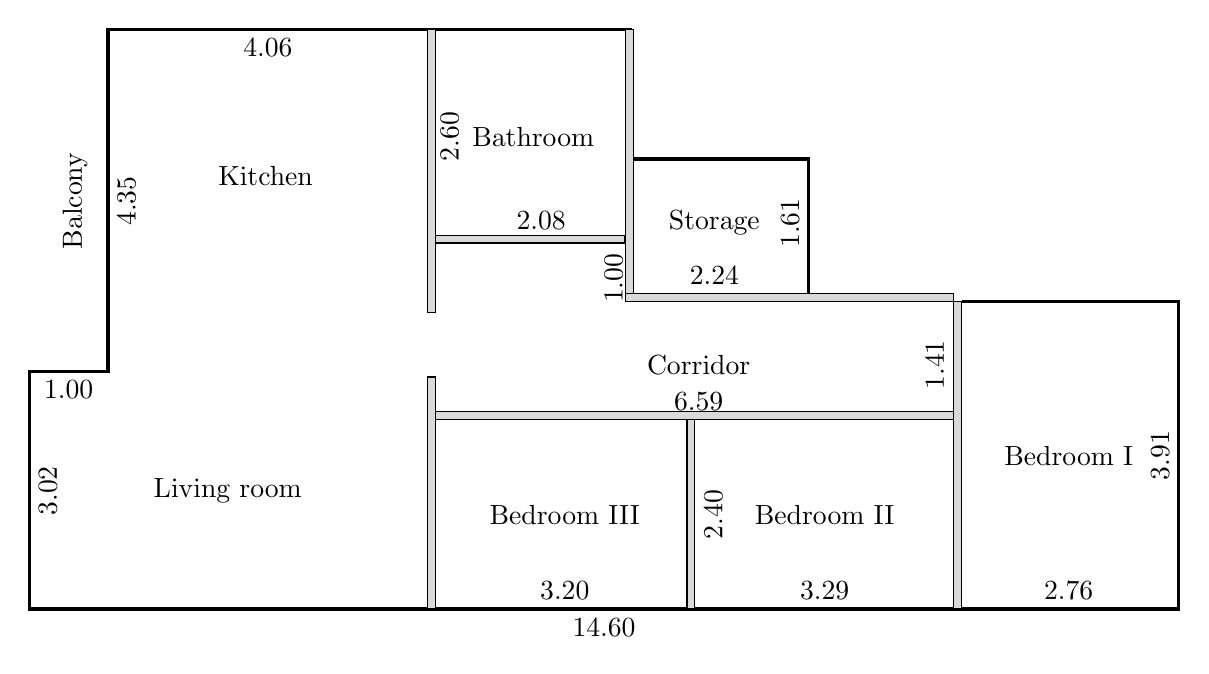
\begin{tikzpicture}
  % \draw[help lines] (0,0) grid (15, 7.36);
  % \foreach \x in {0, 1, ..., 15} \node[below, gray!50] at (\x,0){\tiny{\x}};
  % \foreach \y in {1, 2, ..., 7} \node[left, gray!50] at (0,\y){\tiny{\y}};
  \node[below] at (0.5, 3.018) {1.00}; %sofa shorter edge
  \node[right, rotate=90, anchor=north] at (0, 1.5) {3.02}; % sofa
  \node[right, rotate=90, anchor=north] at (1, 5.18) {4.35}; % biggest window
  \node[below] at (3.03, 7.362) {4.06}; % kitchen width
  \node[below] at (7.299, 0) {14.60};   % total length
  \node at (13.2, 1.95) {Bedroom I};
  \node[above] at (13.2, 0) {2.76};
  \node[left, rotate=90, anchor=south] at (14.6, 1.95) {3.91};
  \node at(10.1, 1.2) {Bedroom II};
  \node[above] at (10.1, 0) {3.29};
  \node[right, rotate=90, anchor=north] at (8.45, 1.2) {2.40};
  \node at (6.8, 1.2) {Bedroom III};
  \node[above] at (6.8, 0) {3.20};
  \node at (8.5, 3.1) {Corridor};
  \node[left, rotate=90, anchor=south] at (11.74, 3.1) {1.41};
  \node[above] at (8.5, 2.4) {6.59};
  \node[left, rotate=90, anchor=south] at (7.66, 4.2) {1.00};
  \node at (6.4, 6) {Bathroom};
  \node[above] at (6.5, 4.7) {2.08};
  \node[right, rotate=90, anchor=north] at (5.1, 6) {2.60};
  \node at (3, 5.5) {Kitchen};
  \node at (2.52, 1.5) {Living room};
  \node at (8.7, 4.9) {Storage};
  \node[above] at (8.7, 4) {2.24};
  \node[left, rotate=90, anchor=south] at (9.9, 4.9) {1.61};
  \node[rotate=90, anchor=north] at (0.3, 5.18) {Balcony};

  \draw[very thick] (7.657, 7.362) -- (1, 7.362) -- (1, 3.018) -- (0, 3.018) -- (0, 0) -- (14.598, 0) -- (14.598, 3.909) -- (11.847, 3.909);
  \draw[very thick] (7.657, 5.717) -- (9.895, 5.717) -- (9.895, 4.009);
  % living room, bathroom edge
  \draw[fill=gray!30] (5.057, 7.362) rectangle (5.157, 3.762);
  % living room, bedroom edge
  \draw[fill=gray!30] (5.057, 2.947) rectangle (5.157, 0);
  
  \draw[fill=gray!30] (5.157, 2.403) rectangle (11.739, 2.503);
  \draw[fill=gray!30] (8.352, 2.403) rectangle (8.453, 0);
  \draw[fill=gray!30] (11.739, 3.909) rectangle (11.839, 0);
  \draw[fill=gray!30] (11.739, 3.909) rectangle (7.57, 4.009);
  \draw[fill=gray!30] (7.57, 4.009) rectangle (7.67, 7.362);
  \draw[fill=gray!30] (5.157, 4.649) rectangle (7.557, 4.749);
\end{tikzpicture}
\end{document}
